\documentclass[12pt, aspectratio=169]{beamer}

\usepackage{color}
\usepackage[utf8]{inputenc}
\usepackage{graphicx}
\usepackage{tikz}
\usepackage[T1]{fontenc}
\usepackage{caption}
\usepackage{wrapfig}
\usepackage{xurl}
\usepackage{animate}

\usepackage{amsmath}
\usepackage{amssymb}
\usepackage{amsthm}
\usepackage{babel}[ngerman]
\usepackage{hyperref}
\usepackage{colonequals}
\usepackage{xfrac}
\usepackage{tikz}
\usepackage{tikz-cd}

\usepackage{graphicx}
\usepackage{caption}

\captionsetup[figure]{labelformat=empty}
\setbeamertemplate{section in toc}[square]
\usefonttheme[onlymath]{serif}

\usetheme{Singapore}
\usecolortheme{default}
\usefonttheme{structurebold}
\setbeamerfont{text}{size=\large}
\setbeamertemplate{bibliography item}{\insertbiblabel}

\definecolor{ao}{rgb}{0.0, 0.0, 0.7}


\setbeamercolor{block body alerted}{bg=alerted text.fg!10}
\setbeamercolor{block title alerted}{bg=alerted text.fg!20}
\setbeamercolor{block body}{bg=structure!10}
\setbeamercolor{block title}{bg=structure!20}
\setbeamercolor{block body example}{bg=green!10}
\setbeamercolor{block title example}{bg=green!20}

\newcommand{\nimadd}{\overset{*}{+}}

%\setbeamertemplate{footline}[frame number]
\setbeamertemplate{footline}[text line]{%
  \parbox{\linewidth}{\vspace*{-8pt}\color{ao}\insertshorttitle\hspace{10px}\insertshortauthor\hfill\insertpagenumber}}

\newcommand{\R}[0]{\mathbb{R}}
\newcommand{\N}[0]{\mathbb{N}}
\newcommand{\T}[0]{\mathcal{T}}
\newcommand{\NB}[0]{\mathcal{N}}
\newcommand*{\logeq}{\ratio\Leftrightarrow}
\newcommand*{\longeq}{\ratio\Longleftrightarrow}
\newcommand*{\bigdot}{\mathpalette\bigcdot@{.5}}
\DeclareRobustCommand{\loongrightarrow}{%
\DOTSB\relbar\joinrel\relbar\joinrel\rightarrow
}

\title{Seminarvortrag \\Fundamentalgruppen als Limites diskreter Fundamentalgruppen}
\author[Y. Höll]{Yannik Höll}
\date{12. Juni, 2024}
% \logo{
\includegraphics[keepaspectratio=True, width=30px]{./image/logo.png}}

\beamertemplatenavigationsymbolsempty 

\begin{document}
\begin{frame}[noframenumbering, plain]
	\titlepage
\end{frame}

\begin{frame}
	\frametitle{Einteilung}
	\tableofcontents
\end{frame}

\begin{frame}
    Notation:
        \begin{itemize}
            \item $Y$ ist ein beliebiger topologischer Raum mit Tologie $\mathcal{T}_Y$,
            \item $X$ ist ein beliebiger metrischer Raum mit Metrik $d_X$,
            \item Für $Z_1, Z_2$ topologische Räume ist $C(Z_1, Z_2) := \{f: Z_1 \to Z_2 \: | \: f \text{ stetig}\}$
            \item Für $y \in Y$ ist $\NB_y$ der Nachbarschaftsfilter von $y$ in $Y$,
            \item Für $\varepsilon \in \R_{>0}$ und $x \in X$ ist $B_{\varepsilon}(x)$ die offene Kugel um $x$ mit Radius $\varepsilon$,
            \item Für $n \in \N$, sei $[n] := \{0, 1, \ldots, n\}$,
            \item Für $n,m \in \N$ mit $n \leq m$, sei $[n,m] := \{n, n+1, \ldots, m\}$.
        \end{itemize}        
\end{frame}

\section{Topologische Grundlagen}

\begin{frame}
    \begin{definition}
        Ein \textbf{Weg} in $Y$ ist eine stetige Abbildung von $[0,1]$ nach $Y$ wobei $[0,1]$ die euklidische Metrik von $\R$ übernimmt.
    \end{definition}
    \begin{definition}<2->
        \onslide<2-> {
        Let $\gamma_1, \gamma_2 \in C([0, 1], Y)$ mit selbem Start- und Endpunkt. Eine \textbf{Homotopie} $H\colon [0,1]^2 \to Y$ zwischen $\gamma_1$ und $\gamma_2$ ist eine stetige Abbildung für die gilt
        \begin{align*}
            &\forall s \in [0,1]\colon H(s, 0) = \gamma_1(s) \: \land \: H(s, 1) = \gamma_2(s), \\
            &\forall t\in[0,1]\forall i\in \{1,2\}\colon H(0, t) = \gamma_i(0) \: \land \: H(1, t) = \gamma_i(1).
        \end{align*}
        }
        \onslide<3-> { Die Wege $\gamma_1, \gamma_2$ heißen \textbf{homotop} ($\gamma_1 \sim_H \gamma_2$), falls eine Homotopie $H$ zwischen ihnen existiert. }
        \onslide<4-> { Wenn ein Weg homotop zum konstanten Weg ($[0,1] \to Y, t \mapsto y \in Y$) ist, dann heißt er \textbf{null-homotop}.}
    \end{definition}
\end{frame}


\begin{frame}
    \begin{definition}
        \onslide<1-> {
            Sei $y_0 \in Y$. Die \textbf{Fundamentalgruppe} von $Y$ mit Basispunkt $y_0$ ist definiert als
            \begin{equation*}
            \pi_1(Y, y_0) := (\{\gamma \in C([0,1],Y) \: | \: \gamma(0) = \gamma(1) = y_0\}/_{\sim}, \: *)
            \end{equation*}
        }
        \onslide<2-> {
        wobei 
        \begin{align*} 
          &*\colon C([0,1], Y) \times C([0,1], Y) \to C([0,1], Y), \\
          &(\gamma_1, \gamma_2) \mapsto \left(t \mapsto \begin{cases}
          \gamma_1(2t),   &t \in [0, {1 \over 2}], \\
          \gamma_2(2t-1), &t \in [{1 \over 2}, 1],
            \end{cases}\right)
        \end{align*}
        die \textbf{Konkatenation} von Pfaden ist. 
        Da nur Schleifen mit dem selben Basispunkt betrachtet werden, kann man belibiege Elemente von $\pi_1(Y, y_0)$ konkatenieren.
        }    
    \end{definition}
\end{frame}

\begin{frame}
\begin{definition}
    \begin{enumerate}
        \item $Y$ \textbf{zusammenhängend} $\;:\Longleftrightarrow\; \forall A,B \in \T_Y\colon (A \cap B = \emptyset \: \land \: Y = A \cup B) \Rightarrow (A = \emptyset \: \lor \: B = \emptyset)$,
        \item $Y$ \textbf{weg-zusammenhängend} $\;:\Longleftrightarrow\; \forall x,y \in Y \exists\gamma \in C([0,1], Y)\colon \gamma(0) = x \: \land \: \gamma(1) = y$,
        \item $Y$ \textbf{lokal weg-zusammenhängend} $\;:\Longleftrightarrow$ \\ $\forall y \in Y\forall U \in \NB_y\exists V\in \NB_y\colon V \subseteq U \: \land \: V$ (weg-)zusammenhängend,
        \item $Y$ \textbf{semi-lokal einfach zusammenhängend} (s.l.s.c) $\: :\Longleftrightarrow$ \\ $\forall y\in Y\exists U \in \NB_y\colon$ Jede Schleife in $U$ ist null-homotop in $Y$
    \end{enumerate}
\end{definition}
\end{frame}

\begin{frame}
Uniforme Bediengungen für metrische Räume:    
\begin{definition}
    \begin{enumerate}
        \item $X$ \textbf{uniform lokal weg-zusammenhängend} (u.l.p.c.) $\: :\Longleftrightarrow$ \\ $\forall \varepsilon \in \R_{>0} \exists \delta \in \R_{>0}\forall x \in X\colon \forall x_1, x_2 \in B_{\delta}(x)\exists \gamma \in C([0,1], B_{\varepsilon}(x))\colon$ \\ $\gamma(0) = x_1 \: \land \: \gamma(1) = x_2$,
        \item $X$ \textbf{uniform semi-lokal einfach zusammenhängend} (u.s.l.s.c) $\: :\Longleftrightarrow$ \\ $\exists \varepsilon \in \R_{>0}\forall x\in X\colon$ Jede Schleife in $B_{\varepsilon}(x)$ ist null-homotop in $X$
        \end{enumerate}
\end{definition}
\end{frame}

\begin{frame} \frametitle{Lemma von Lebesgue}
    \begin{lemma}
        Sei $\mathcal{U}$ eine offene Überdeckung von $X$. Wenn $X$ kompakt ist, dann existiert ein $\delta \in \R_{>0}$, sodass
        \begin{equation*}
          \forall A \in \mathcal{P}(X)\colon d(A) < \delta \Rightarrow (\exists U \in \mathcal{U}\colon A \subseteq U),
        \end{equation*}
        wobei $d\colon \mathcal{P}(X) \to [0, \infty), \: A \mapsto \sup \{ d_X(a_1, a_2) \: | \: a_1,a_2\in A \}$ der Durchmesser einer Teilmenge von $X$ ist.
        Diese Zahl $\delta$ wird dann als \textbf{Lebesguezahl} bezeichnet.
    \end{lemma}
\end{frame}

\section{Diskretisierung der Fundamentalgruppe}

\begin{frame}
    \begin{definition} \label{def:discrete-path}
        Sei $\theta \in \R_{>0}$ und $n \in \N$. Ein \textbf{diskreter Weg} ($\theta$-Weg) mit der Länge $n$ ist eine Abbildung $Z: [n] \to X$,
        welche $\theta$-Lipschitz ist (mit der euklidischen Metrik geerbt von $\R$), also
        \begin{equation}
          \forall n_1, n_2 \in [n]\colon d_X(Z(n_2), Z(n_1)) \leq \theta |n_2 - n_1|.
        \end{equation}
        Eine weitere Möglickeit der Definition ist als Folge $(z_i)_{i=0}^n$ mit $z_i \in X$ und
        \begin{equation}
          \forall i \in \{0, 1, \ldots, n-1\} \colon d_X(z_i, z_{i+1}) \leq \theta.
        \end{equation}
      
        Sei $m \in \N$ mit $m \geq n$ und sei $Z'\colon [m] \to X$ ein diskreter Weg. $Z'$ heißt \textbf{Lazification} von $Z$ wenn eine surjektive, monotone Abbildung 
        $f\colon [m] \to [n]$, sodass $Z' = Z \circ f$. 
      \end{definition}
\end{frame}

\begin{frame}
    \begin{definition}
        Sei $\theta \in \R_{>0}$, $n,m \in \N$ und seien $Z_1\colon [n] \to X, Z_2: [n] \to X$ diskrete $\theta$-Wege in $X$, mit selbem Start- und Endpunkt.
        Eine \textbf{$\theta$-Gitterhomotopie} ist eine $\theta$-Lipschitz Abbildung $H\colon [n] \times [m] \to X$, sodass
        \begin{align*}
            &H(\cdot, 0) = Z_1 \: \land \: H(\cdot, m) = Z_2, \\
            &\forall t\in [m]\colon H(0,t) = Z_1(0) = Z_2(0) \: \land \: H(n,t) = Z_1(n) = Z_2(n),
        \end{align*}
        wobei das Produkt $[n] \times [m]$ ein metrischer Raum mit der $\ell_1$-Metrik ist.
    \end{definition}

    \begin{definition}
        Sei $\theta \in \R_{>0}$ und seien $Z_1, Z_2$ diskrete $\theta$-Wege. $Z_1$ und $Z_2$ heißen \textbf{$\theta$-homotop} ($Z_1 \sim_{\theta} Z_2$)
        wenn Lazifications $Z_1'$ von $Z_1$ und $Z_2'$ von $Z_2$ mit der gleichen Länge existieren und eine $\theta$-Gitterhomotopie zwischen $Z_1'$ und $Z_2'$.
    \end{definition}
\end{frame}

\begin{frame}
    \begin{block}{Bemerkung}
        Seien $(x_0, x_1, \ldots, x_n)$ und $(y_0, y_1, \ldots, y_n)$ mit $n \in \N, y_0 = y_n$ und $x_0 = x_n$ zwei geschlossene $\theta$-Wege in $X$. 
        Eine nützliche Darstellung einer $\theta$-Gitterhomotopie ist die folgende Matrix  
        \begin{equation*}
            \begin{matrix}
            x_0 & x_1 & x_2 & \cdots & x_n \\
            z_0^1 & z_1^1 & z_2^1 & \cdots & z_n^1 \\
            \vdots & \vdots & \vdots & \vdots & \vdots \\
            z_0^{t} & z_1^{t} & z_2^{t} & \cdots & z_n^{t} \\
            y_0 & y_1 & y_2 & \cdots & y_n \\
            \end{matrix}
        \end{equation*}
        in welcher die Zeilen $\theta$-Schleifen in $X$ sind und die Spalten $\theta$-Wege in $X$ und $t\in \N$.
    \end{block}
\end{frame}

\begin{frame}
    \begin{definition}
        Sei $\theta \in \R_{>0}$ und $x_0 \in X$. $\mathcal{C}_{\theta}(X, x_0)$ ist die Menge aller geschlossenen, diskreten $\theta$-Wege in $X$ mit Basispunkt $x_0$. 
        Seien nun $x, y \in \mathcal{C}_{\theta}(X, x_0)$, also    
        \begin{equation*}
            x = (x_0, x_1, \ldots, x_n = x_0), \: y = (y_0, y_1, \ldots, y_m = y_0)
        \end{equation*} mit $x \in X^{n+1}$ und $y \in X^{m+1}$.
        
        Definiere nun die \textbf{Konkatenation} von diskreten Wegen 
        $*\colon \mathcal{C}_{\theta}(X, x_0) \times \mathcal{C}_{\theta}(X, x_0) \to \mathcal{C}_{\theta}(X, x_0), (x, y) \mapsto x * y$, wobei
        \begin{equation*}
            x * y = (x_0, x_1, \ldots, x_n = y_0, y_1, \ldots, y_m),
        \end{equation*}
        also $x * y\colon [n+m] \to X, t \mapsto \begin{cases}
            x_t, &t \in [n], \\
            y_{t-n}, &t \in [n,n+m].
        \end{cases}$
    \end{definition}
\end{frame}

\begin{frame}
    \begin{lemma}<1-> \label{lem:discrete-homotopy}
        Sei $\theta \in \R_{>0}$, dann ist die $\theta$-Gitterhomotopierelation $\sim_{\theta}$ auf $\mathcal{C}_{\theta}(X, x_0)$ eine Äquivalenzrelation.
    \end{lemma}

    \begin{definition}<2->
        Sei $\theta \in \R_{>0}$ und sei $x_0 \in X$. $\pi_{1,\theta}(X, x_0) := (\mathcal{C}_{\theta}(X, x_0)/_{\sim_{\theta}}, *)$ heißt \textbf{diskrete Fundamentalgruppe} mit der Skala $\theta$.
        Die Gruppenoperation ist die Konkatenation $*\colon \pi_{1,\theta}(X, x_0) \times \pi_{1,\theta}(X, x_0) \to \pi_{1,\theta}(X, x_0), ([x]_{\theta}, [y]_{\theta}) \mapsto [x * y]_{\theta}$.
    \end{definition}
    
    \begin{Satz}<3->
        Sei $\theta \in \R_{>0}$ und $x_0 \in X$. Die diskrete Fundamentalgruppe $\pi_{1,\theta}(X, x_0)$ ist wohldefiniert.
    \end{Satz}
\end{frame}

\begin{frame}
    \begin{block}{Bemerkung}
        Für $\theta' \leq \theta$ existiert ein natürlicher Homomorphismus $\pi_{1,\theta'}(X, x_0) \to \pi_{1,\theta}(X, x_0)$,
        weil jeder $\theta'$-Weg auch ein $\theta$-Weg ist und jede $\theta'$-Gitterhomotopie auch eine $\theta$-Gitterhomotopie ist.
    \end{block}
      
    \begin{block}{Bemerkung}
        Jeder geschlossene $\theta$-Weg mit einer Länge $\leq 4\theta$ ist $\theta$-nullhomotop.
    \end{block}
\end{frame}

\section{Inverser Limes}

\begin{frame}
    \begin{definition}
        Sei $(I, \leq)$ eine halbgeordnete, gerichtete Menge, 
        $(G_i)_{i\in I}$ eine Familie von Gruppen und sei $(\varphi_{ij})_{i,j \in I, i \leq j}$ eine Familie von Homomorphismen 
        $\varphi_{ij}\colon G_j \to G_i$, sodass für alle $i,j,k \in I$ mit $i \leq j \leq k$
        \begin{equation*}
            \varphi_{ii} = \text{id}_{G_i} \: \land \: \varphi_{ij} \circ \varphi_{jk} = \varphi_{ik}.
        \end{equation*}
        Dann ist der \textbf{inverse Limes} der Familie $(G_i)_{i\in I}$ bezüglich der Homomorphismen $(\varphi_{ij})_{i,j \in I, i \leq j}$ definiert als
        \begin{equation*}
            \varprojlim_{i\in I} G_i := \left\{(g_i)_{i\in I} \in \prod_{i\in I} G_i \: \middle| \: \forall i,j \in I, i \leq j: \varphi_{ij}(g_j) = g_i\right\}
        \end{equation*}
        mit der Operation $((g_i)_{i\in I}, (h_i)_{i\in I}) \mapsto (g_i \cdot h_i)_{i\in I}$.
    \end{definition}
\end{frame}

\begin{frame}
    \begin{definition}<1->
        Sei $\theta \in \R_{>0}$, $\gamma\colon [0,1] \to X$ ein stetiger Weg in $X$ und seien $0 = t_0 \leq t_1 \leq \ldots \leq t_n = 1$ mit $n \in \N$.
        
        Die Folge $(\gamma(t_i))_{i=0}^n$ heißt \textbf{$\theta$-Diskretisierung} von $\gamma$, wenn für alle $i \in \{1, \ldots, n\}$ gilt
        \begin{equation*}
            d_X(\gamma(t_{i}), \gamma(t_{i-1})) \leq \theta.
        \end{equation*}
        Für die Diskretisierung von $\gamma$ schreibt man $\widehat{\gamma}^{\theta}_{(t_0, \ldots, t_n)}$.
    \end{definition}

    \begin{lemma}<2->\label{lem:discretization}
        Sei $\theta \in \R_{>0}$. Jeder stetige Weg erzeugt eine eindeutige $\theta$-Diskretisierung bis auf $\theta$-Gitterhomotopie. 
        Wenn die Wege $\alpha, \beta\colon [0,1] \to X$ homotop sind, dann sind alle $\theta$-Diskretisierungen 
        $\widehat{\alpha}^{\theta}_{(t_0, \ldots, t_n)}$, $\widehat{\beta}^{\theta}_{(t_0', \ldots, t_m')}$ $\theta$-homotop ($n,m \in \N$).
    \end{lemma}
\end{frame}

\begin{frame}
    \begin{Theorem}<1-> \label{thm:isomorphism}
        Wenn $X$ \textbf{uniform lokal weg-zusammenhängend} und \textbf{uniform semi-lokal einfach zusammenhängend} ist, 
        dann ist die Diskretisierungsabbildung $\: \widehat{\cdot} : \pi_{1,\theta}(X, x_0) \to \varprojlim \pi_{1,\theta}(X, x_0)$ ein Gruppenisomorphismus.
    \end{Theorem}

    \begin{Folgerung}
        Wenn $X$ \textbf{lokal weg-zusammenhängend}, \textbf{semi-lokal einfach zusammenhängend} und \textbf{kompakt} ist, dann ist die Diskretisierungsabbildung 
        $\hspace*{2px}\widehat{\cdot}\hspace*{2px}\colon \pi_1(X, x_0) \to \varprojlim \pi_{1,\theta}(X, x_0)$
        ein Gruppenisomorphismus.
    \end{Folgerung}
\end{frame}

\begin{frame}
    \begin{figure}
        \centering
        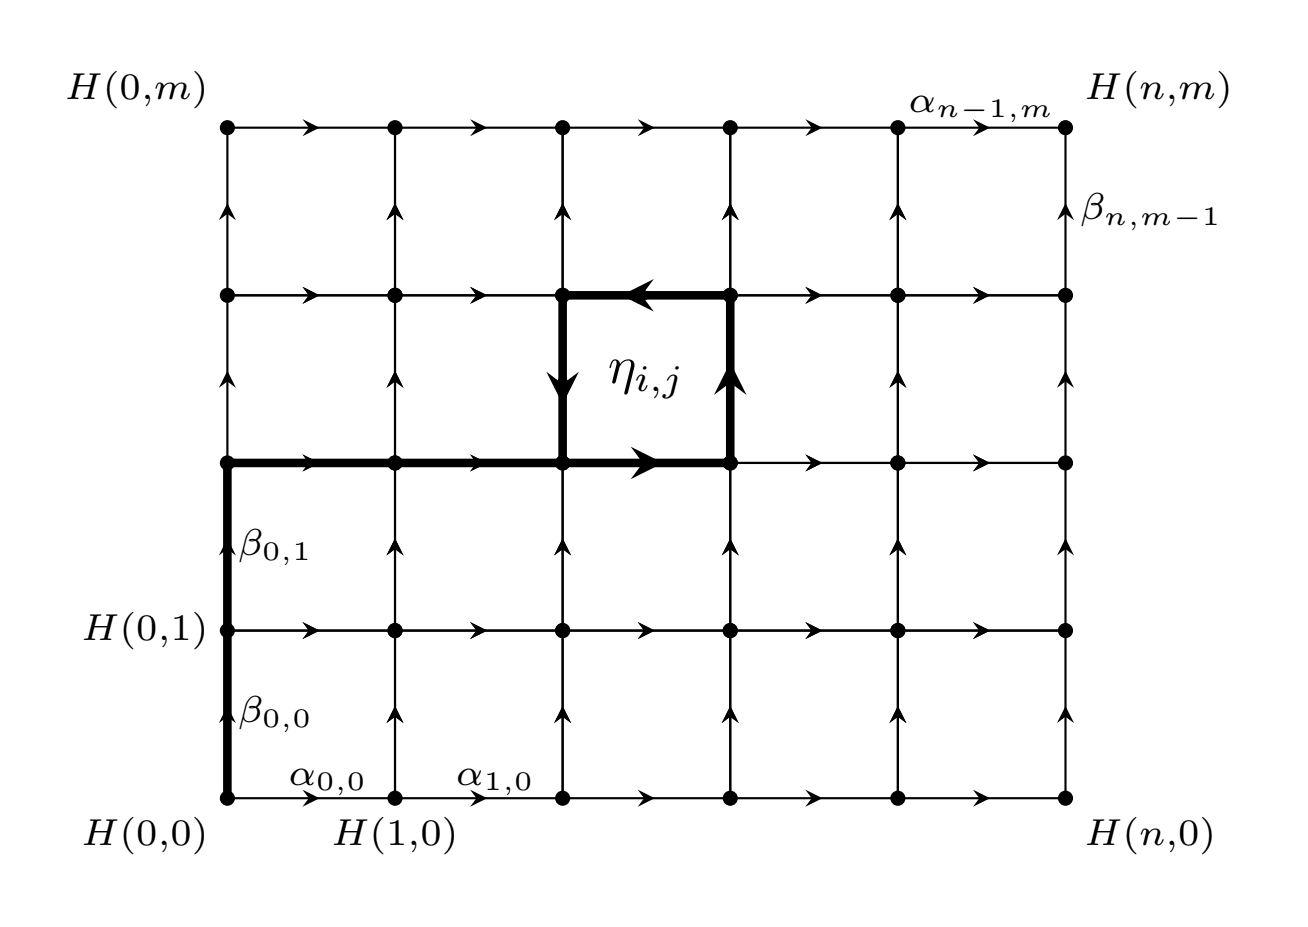
\includegraphics[width=0.7\textwidth]{plot/ProofPic.png}
        \caption{Konstruktion einer stetigen Homotopie \cite{vigolo2018fundamental}}        
    \end{figure}
\end{frame}

\section{Gegenbeispiele von metrischen Räumen}

\begin{frame}
    \begin{figure}
        \centering
        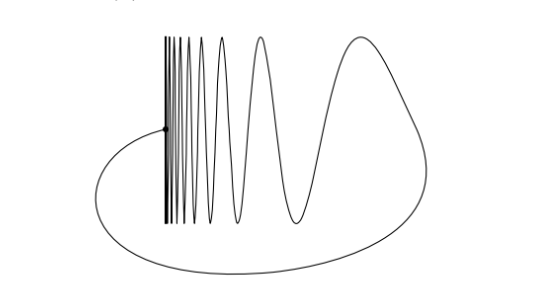
\includegraphics[width=0.5\textwidth]{ex1.png}
        \caption{Gegenbeispiel Injektivitität \cite[p. 8]{vigolo2018fundamental}}
    \end{figure}
\end{frame}

\section{Quellen}

\begin{frame}[allowframebreaks, noframenumbering]
    \nocite{*}
	\hfill
    \bibliographystyle{unsrt}
    \bibliography{presentation-ref}
\end{frame}


\end{document}